\documentclass[12pt,letterpaper,oneside,reqno]{amsart}
\usepackage{amsfonts}
\usepackage{amsmath}
\usepackage{amssymb}
\usepackage{amsthm}
\usepackage{float}
\usepackage{mathrsfs}
\usepackage{colonequals}
\usepackage[font=small,labelfont=bf]{caption}
\usepackage[left=1in,right=1in,bottom=1in,top=1in]{geometry}
\usepackage[pdfpagelabels,hyperindex,colorlinks=true,linkcolor=blue,urlcolor=magenta,citecolor=green]{hyperref}
\usepackage{setspace}
\usepackage{graphicx}
\usepackage{spverbatim}
\onehalfspacing
\emergencystretch=1em

\linespread{1.25}

\newcommand \anglePower [2]{\langle #1 \rangle \sp{#2}}
\newcommand \bernoulli [2][B] {{#1}\sb{#2}}
\newcommand \curvePower [2]{\{#1\}\sp{#2}}
\newcommand \coeffA [3][A] {{\mathbf{#1}} \sb{#2,#3}}
\newcommand \polynomialP [4][P]{{\mathbf{#1}}\sp{#2} \sb{#3}(#4)}

% ordinary derivatives
\newcommand \derivative [2] {\frac{d}{d #2} #1}                              % 1 - function; 2 - variable;
\newcommand \pderivative [2] {\frac{\partial #1}{\partial #2}}               % 1 - function; 2 - variable;
\newcommand \qderivative [1] {D_{q} #1}                                      % 1 - function
\newcommand \nqderivative [1] {D_{n,q} #1}                                   % 1 - function
\newcommand \qpowerDerivative [1] {\mathcal{D}_q #1}                         % 1 - function;
\newcommand \finiteDifference [1] {\Delta #1}                                % 1 - function;
\newcommand \pTsDerivative [2] {\frac{\partial #1}{\Delta #2}}               % 1 - function; 2 - variable;

% high order derivatives
\newcommand \derivativeHO [3] {\frac{d^{#3}}{d {#2}^{#3}} #1}                % 1 - function; 2 - variable; 3 - order
\newcommand \pderivativeHO [3]{\frac{\partial^{#3}}{\partial {#2}^{#3}} #1}
\newcommand \qderivativeHO [2] {D_{q}^{#2} #1}                               % 1 - function; 2 - order
\newcommand \qpowerDerivativeHO [2] {\mathcal{D}_{q}^{#2} #1}                % 1 - function; 2 - order
\newcommand \finiteDifferenceHO [2] {\Delta^{#2} #1}                         % 1 - function; 2 - order
\newcommand \pTsDerivativeHO [3] {\frac{\partial^{#3}}{\Delta {#2}^{#3}} #1} % 1 - function; 2 - variable;

\newtheorem{thm}{Theorem}[section]
\newtheorem{cor}[thm]{Corollary}
\newtheorem{lem}[thm]{Lemma}
\newtheorem{examp}[thm]{Example}

\numberwithin{equation}{section}

\title[Diffie-Hellman Key Exchange via REST]
{Diffie-Hellman Key Exchange via REST}
\author[Petro Kolosov]{Petro Kolosov}
\email{kolosovp94@gmail.com}
\keywords{
    Diffie-Hellman Key Exchange, DH key exchange, REST
}
\urladdr{https://razumovsky.me}
\subjclass[2010]{26E70, 05A30}
\date{\today}
\hypersetup{
    pdftitle={Diffie-Hellman Key Exchange via REST},
    pdfsubject={
        Diffie-Hellman Key Exchange, DH key exchange, REST
    },
    pdfauthor={Petro Kolosov},
    pdfkeywords={
        Diffie-Hellman Key Exchange, DH key exchange, REST
    }
}
\begin{document}
    \begin{abstract}
        Discussion on Diffie-Hellman Key Exchange and its implementation via REST.
    \end{abstract}

    \maketitle

    \tableofcontents


    \section{Introduction} \label{sec:introduction}
    Diffie--Hellman (DH) protocol is a method of asymmetric exchange
    of the cryptographic keys for a group of two or more participants,
    developed in 1976 by cryptographers Ralph Merkle, Whitfield Diffie and Martin Hellman.
    In contrast to the symmetric key exchange,
    the Diffie\textendash Hellman protocol eliminates the direct transfer of the shared secret
    between the participants so that each participant computes a shared secret with his own private-public key pair.
    The Diffie\textendash Hellman protocol is based on a one-way function of the form

    \begin{equation}
        A = G ^ a \bmod P \label{eq:equation}
    \end{equation}

    where $A$ is the user's public key,
    $a$ is the user's private key,
    $P=2Q+1$ is modulus, such that 2048 bits safe-prime because $Q$ is also prime,
    $G$ is generator such that $G$ is primitive root modulo $P$.
    We say that $G$ is primitive root modulo $P$ if for each $1 \leq a \leq P - 1$ the $A = G ^ a \bmod P$
    is unique and belong to the set $\{1, 2, \dots, P-1\}$.
    The period of such cyclic group $\mathbb{Z}_{P}$ is $P-1$ then.

    Thus, the safety of the Diffie--Hellman protocol is based on the discrete logarithm problem which is unsolvable
    in polynomial time if the constants $G$ and $P$ are chosen correctly.
    Graphically the flow of the Diffie--Hellman protocol can be expressed through the
    analogy with mixing paints as the picture below shows
    \begin{figure}[H]
        \centering
        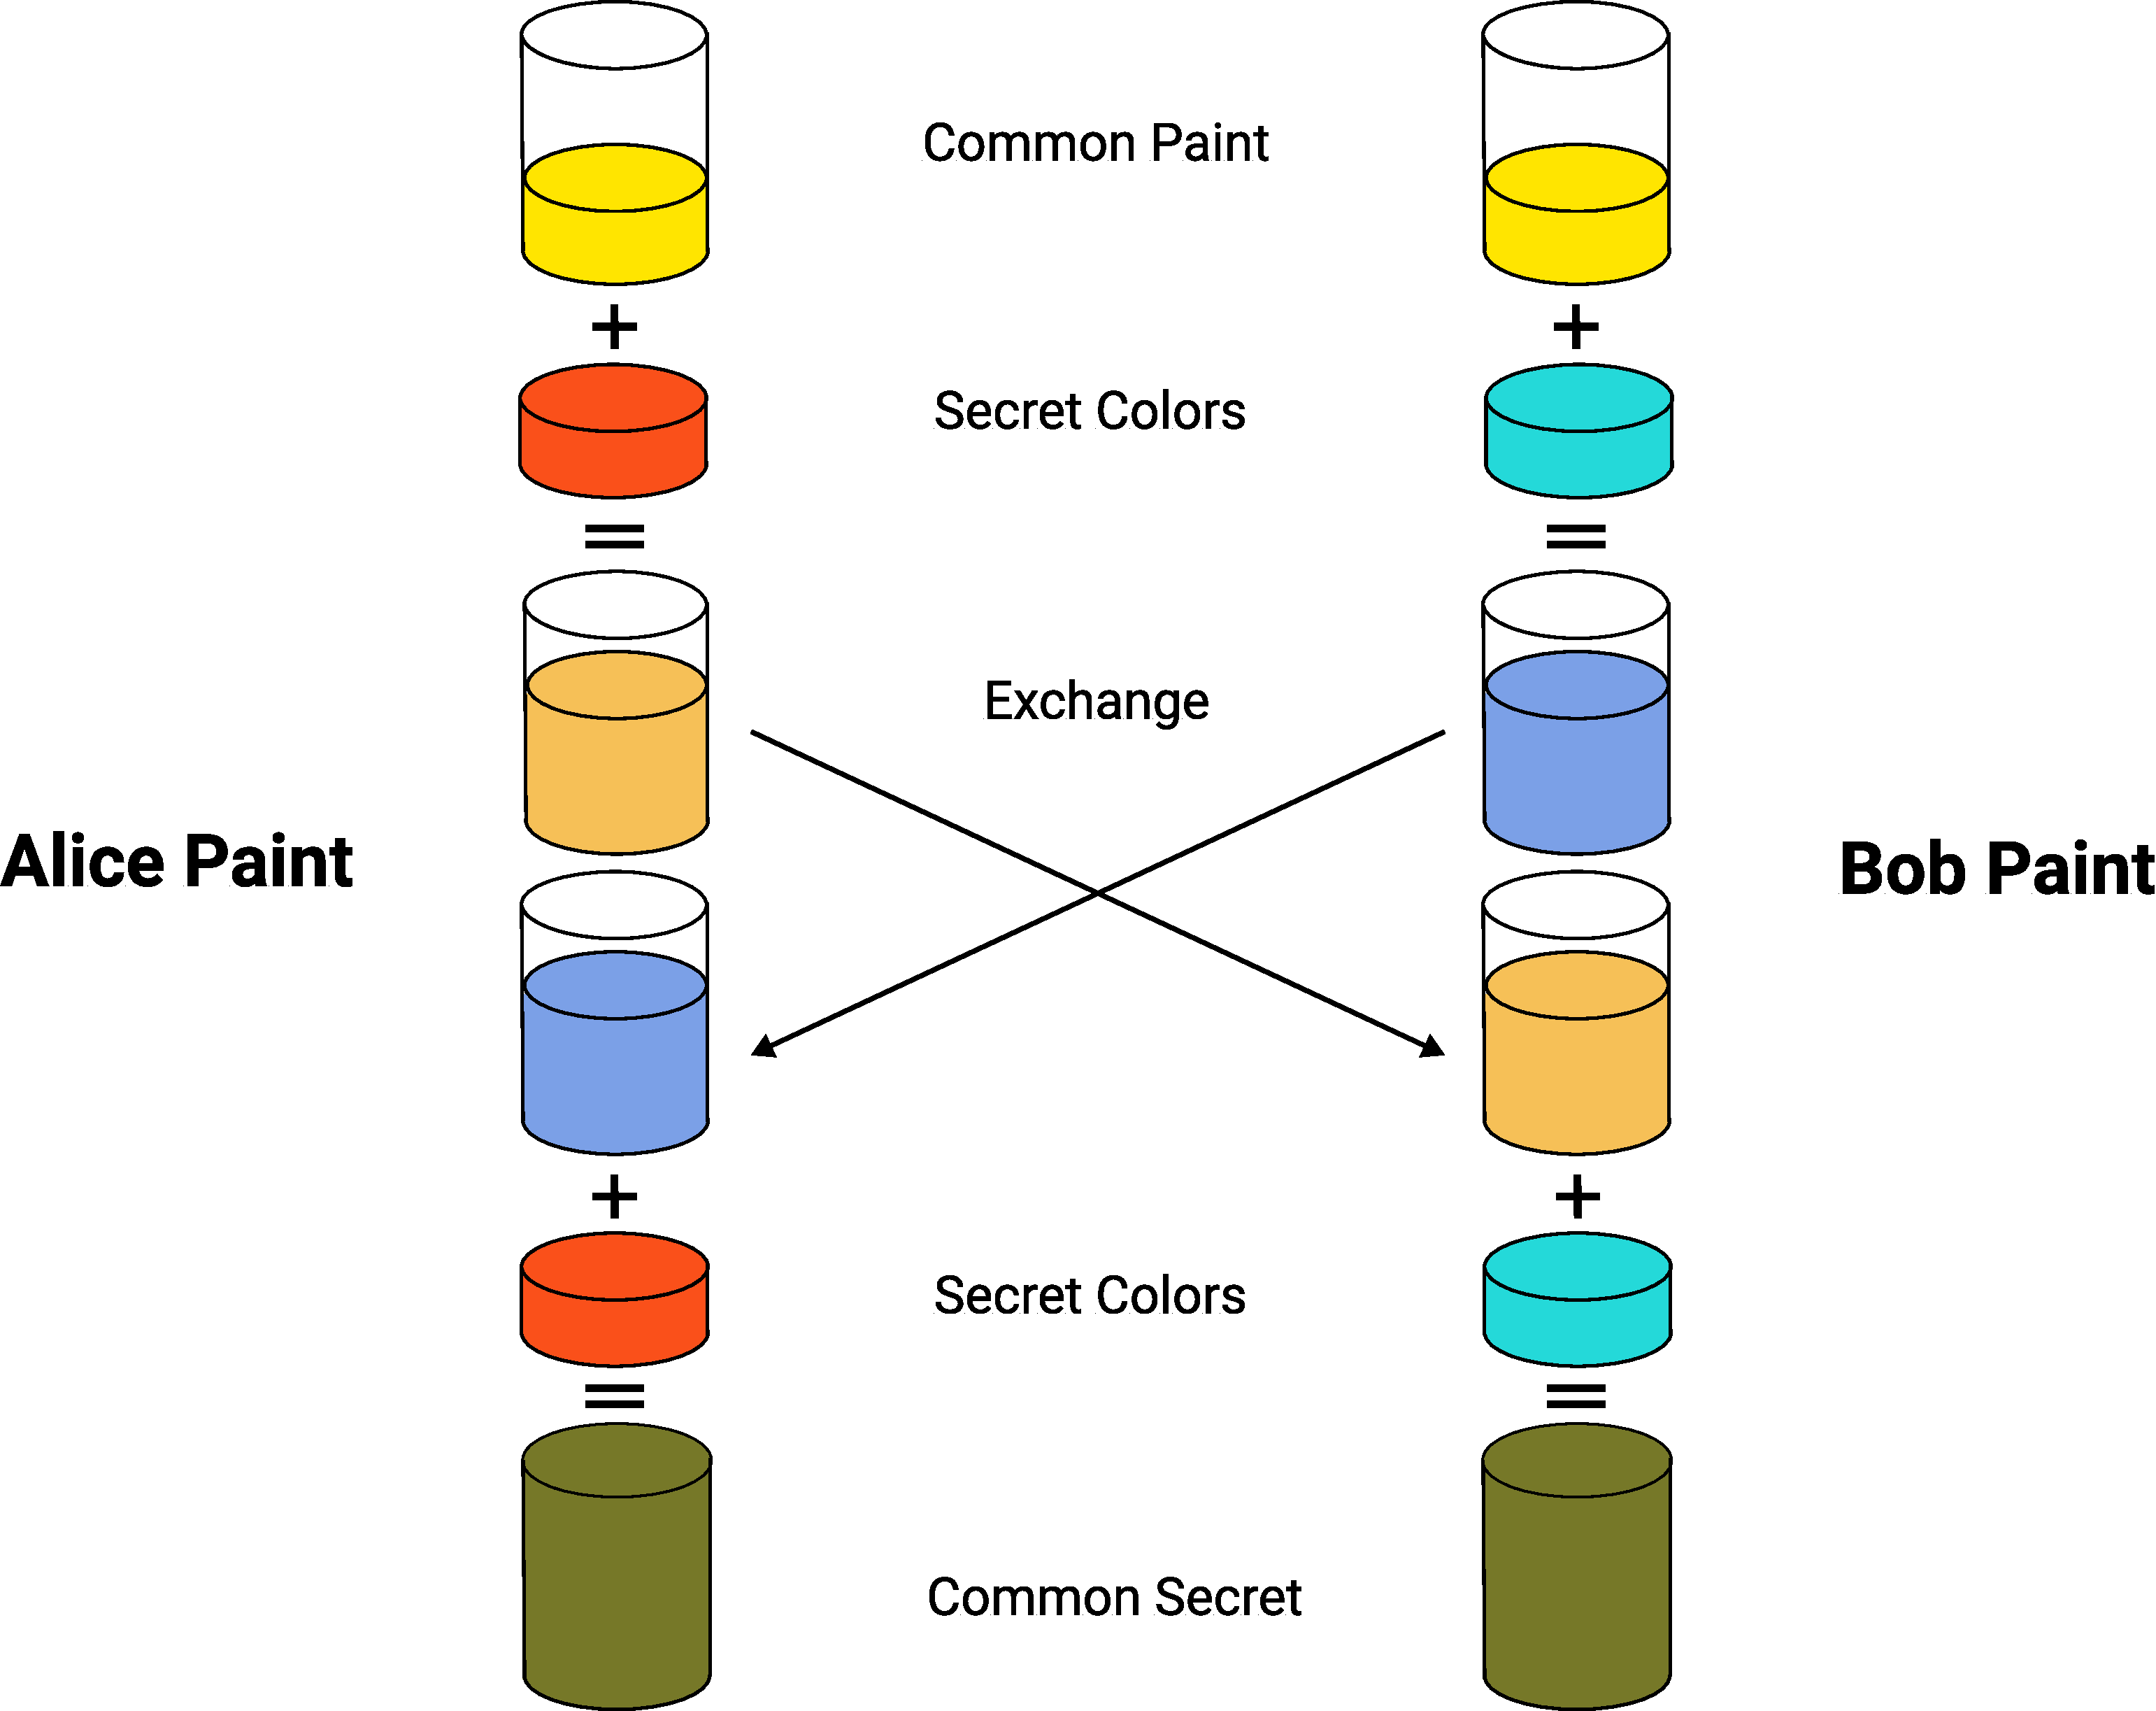
\includegraphics[width=1\textwidth]{Pictures/Diffie_Hellman_keyexchange_concept_diagram}
        ~\caption{Diffie\textendash Hellman key exchange concept diagram.}\label{fig:figure4}
    \end{figure}
    In contrast to the Diffie\textendash Hellman based on discrete logarithm problem, there is an Elliptic Curve Diffie\textendash Hellman
    key exchange, which based on the elliptic curve discrete logarithm problem.
    Although, the idea is quite same, the difference only in that Elliptic Curve Diffie\textendash Hellman ensures the same safety
    as discrete logarithm Diffie\textendash Hellman with lower value of the prime modulus $P$.
    For instance, 521 bit modulus used in Elliptic Curve Diffie\textendash Hellman is equally safe as 2048 bit modulus in
    discrete logarithm Diffie\textendash Hellman.
    To summarize, the flow of Diffie\textendash Hellman key exchange is as follows.
    Given 2048 bits public prime modulus $P$ and generator $G$ such that $G$ is primitive root modulo $P$ then
    \begin{enumerate}
        \item Alice chooses her secret $a$.
        \item Alice sends to Bob her public key $A = G^a \bmod P$.
        \item Bob chooses his secret $b$.
        \item Bob sends to Alice his public key $B = G^b \bmod P$.
        \item Alice computes common secret $s = B^a \bmod P$.
        \item Bob computes common secret $s = A^b \bmod P$.
        \item Alice and Bob have arrived to the same value
        \begin{eqnarray}
            s = A^b \bmod P = G^{ab} \bmod P \\
            s = B^a \bmod P = G^{ba} \bmod P
        \end{eqnarray}
    \end{enumerate}

    \begin{figure}[H]
        \centering
        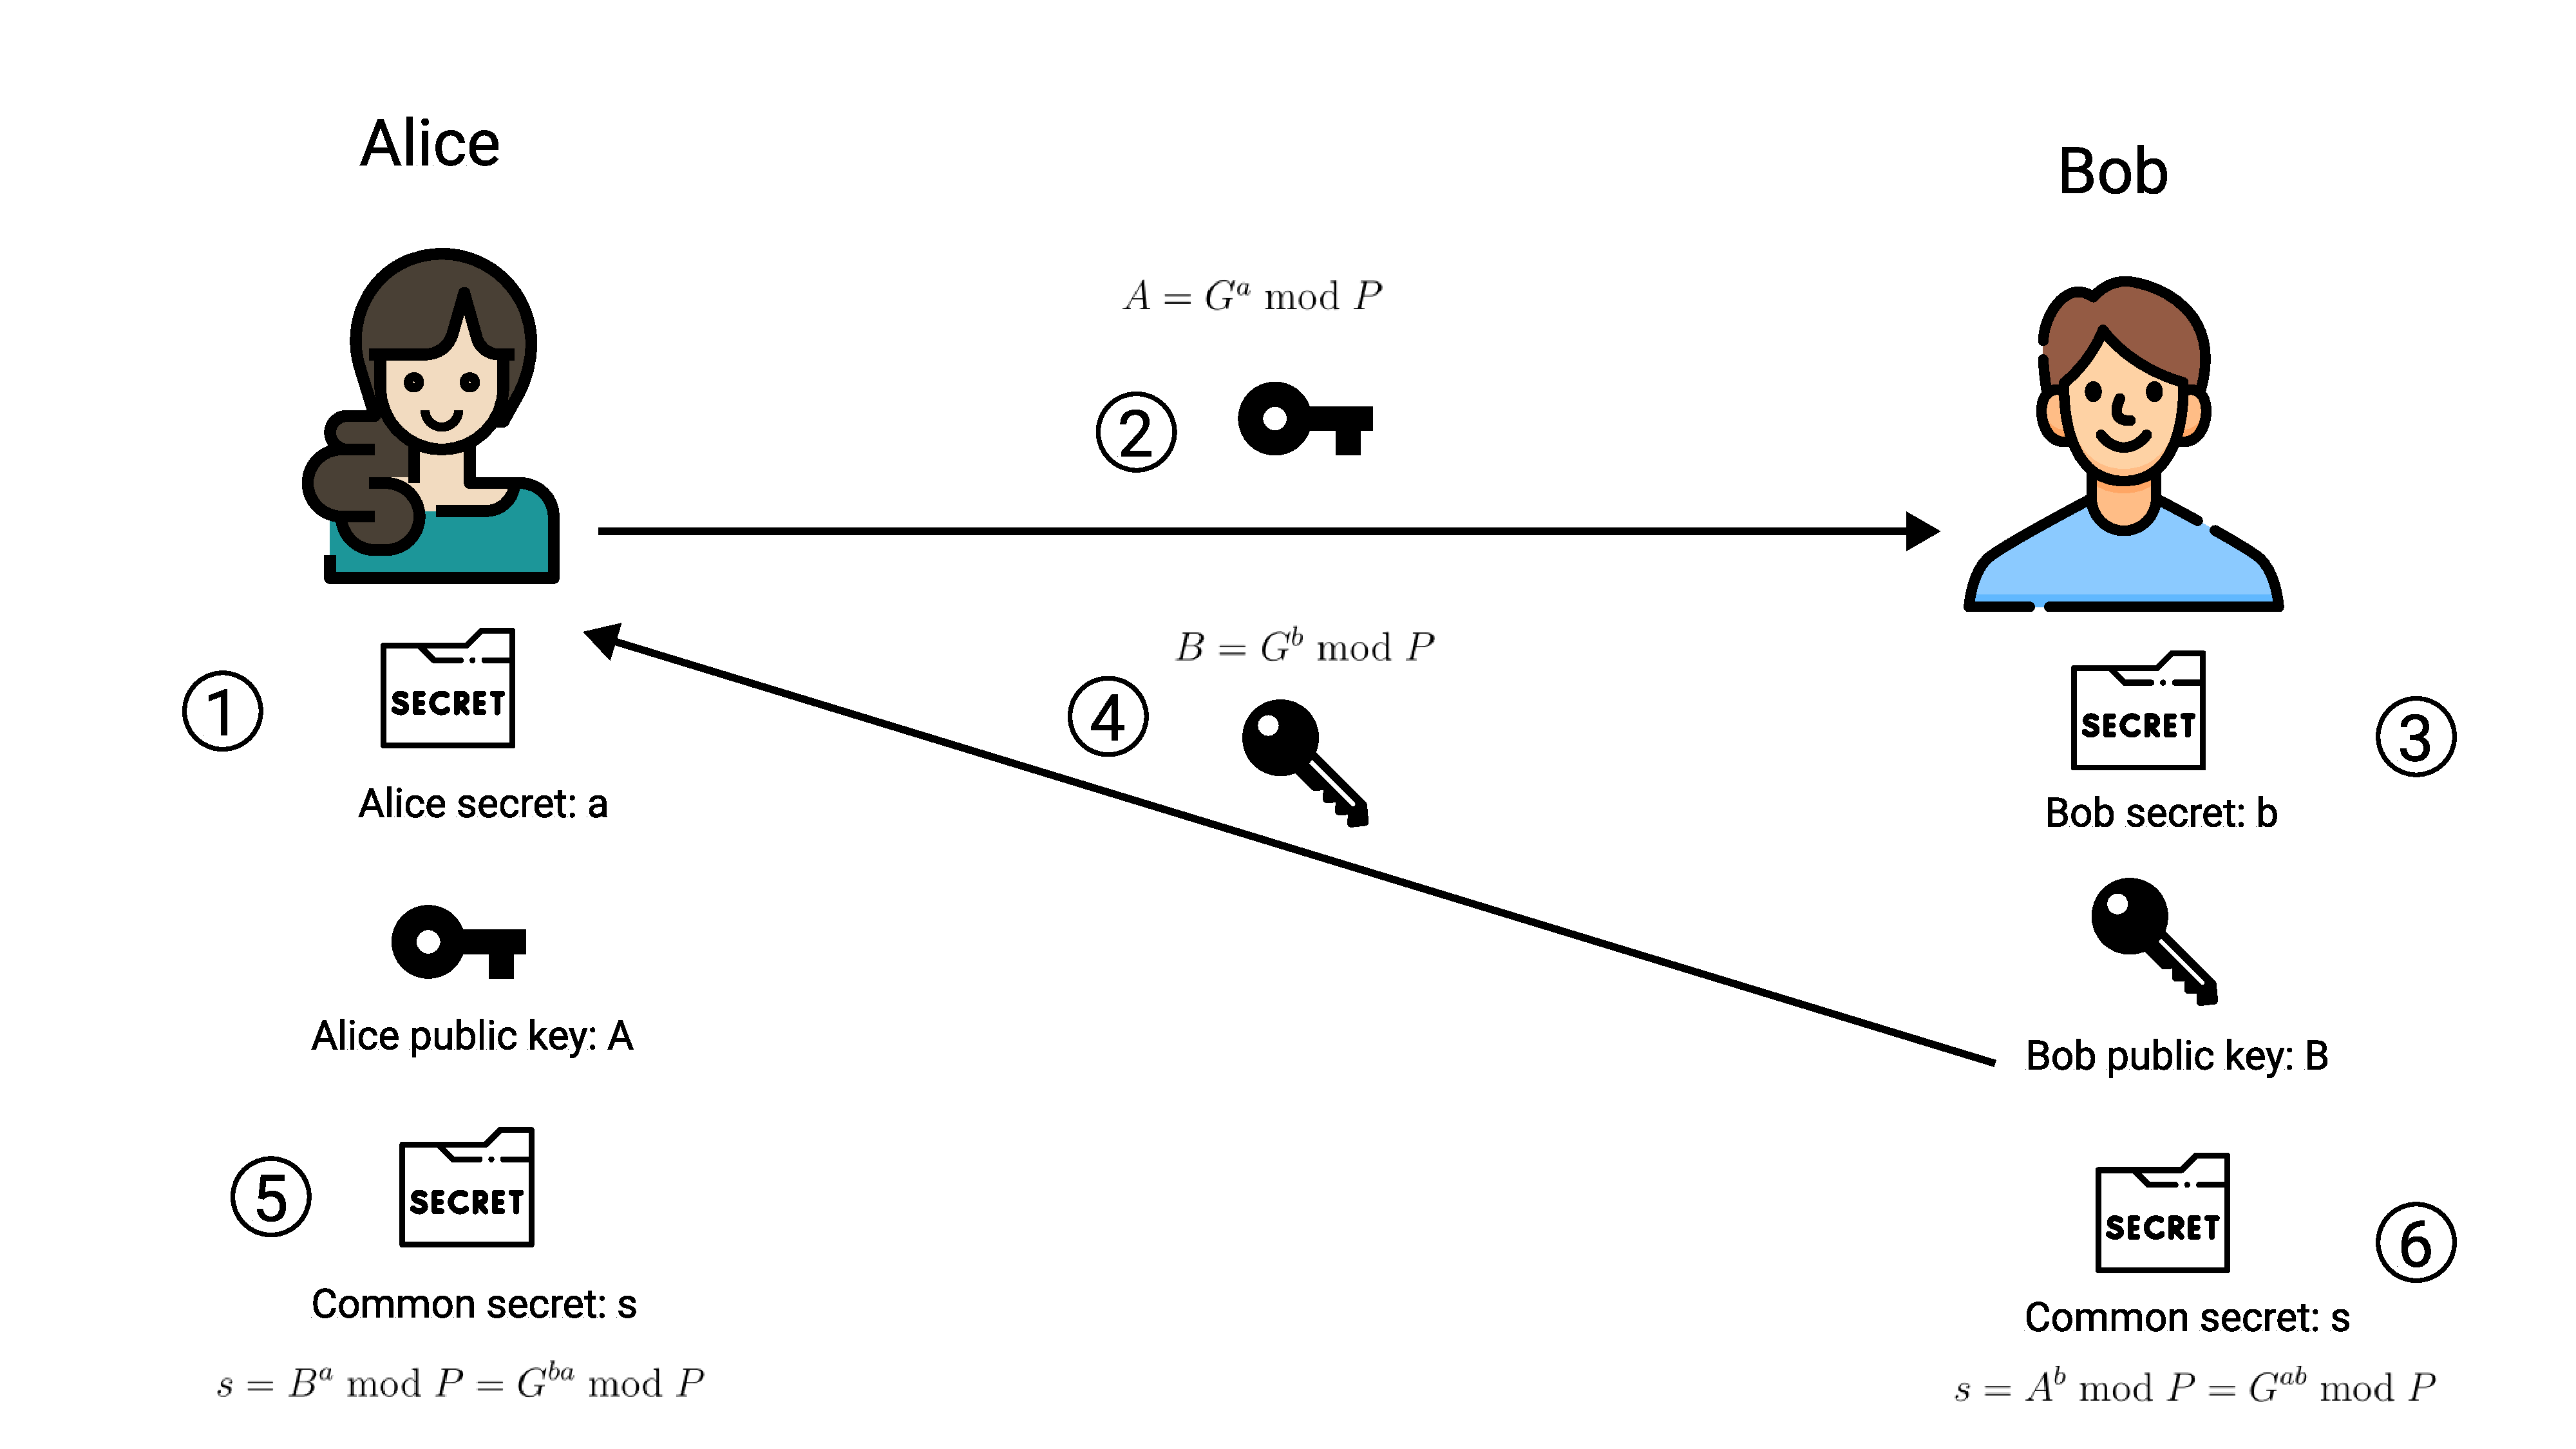
\includegraphics[width=1\textwidth]{Pictures/DH_Key_Exchange}
        ~\caption{Diffie\textendash Hellman key exchange concept diagram.}\label{fig:figure}
    \end{figure}


    \section{Diffie\textendash Hellman key exchange implementation via REST}
    \label{sec:diffie–-hellman-key-exchange-implementation-via-rest}
    Although, the idea of Diffie\textendash Hellman key exchange looks quite simple,
    some remarks on the concrete implementation should be added.
    Firstly, it is necessary to implement the mechanism of key exchange request between two or more parties.
    As it discussed above, each user has his own private-public keys pair, so in order to perform request between parties,
    it should be implemented dedicate REST~\cite{ong2015materials} web--service endpoint,
    for instance the \texttt{POST: api/key-exchange-requests} which takes the request body of the form

    \begin{spverbatim}
{
    "requestedUserId": "3fa85f64-5717-4562-b3fc-2c963f66afa6",
    "publicKey": "RUNLMSAAAAC2lkqYcTGhutQPxcjvoqUELKoy0"
}
\end{spverbatim}

    So, request sender generates on the client side a key pair, keeps private on in the file system and shares the public
    in request to receiver.
    Therefore, the second party has received the key exchange request.
    In order to display all the key exchange requests awaiting the confirmation of decline decisions, it is worth to implement
    another REST endpoint such that \texttt{GET: api/key-exchange-requests}, so that requested party will have the list of
    requests to proceed.
    This endpoint may return the data structure like follows

    \begin{spverbatim}
{
    "keyExchangeRequests": [
        {
            "requestId": "81d314c1-913f-4686-827e-ef2a65ccc370",
            "senderId": "3fa85f64-5717-4562-b3fc-2c963f66afa6",
            "senderPublicKey": "RUNLMSAAAAC2lkqYcTGhutQPxcjvoqUELKoy0"
        }
    ],
    "message": "SUCCESS",
    "success": true
}
\end{spverbatim}

    Finally, requested party should be able to confirm or decline the key exchange request, the
    \texttt{DELETE: api/key-exchange-requests} endpoint should be implemented then.
    The server is able to fetch the request thanks to the body endpoint takes

    \begin{spverbatim}
{
    "requestId": "3fa85f64-5717-4562-b3fc-2c963f66afa6",
    "confirmed": true,
    "publicKey": "string"
}
\end{spverbatim}

    Therefore, an identifier of awaiting request is passed to the server among with boolean value
    indicating the confirmation.
    Under the roof of this operation are also generation of private-public keys pair for the requested party and
    generation of common secret stored in client's file system.
    As result, the initial request sender receives a public key as confirmation from requested party.
    Requested side may get all his public keys via the REST web--service using the resource \texttt{GET: api/public-keys}

    \begin{spverbatim}
{
    "publicKeys": [
        {
            "partnerId": "ae9e10a4-0c7e-4911-8450-4139d4a114a7",
            "partnerPublicKey": "RUNLMSAAAAAbc49wfaZ+QF9J2cu1S66bkp0"
        }
    ],
    "message": "SUCCESS",
    "success": true
}
\end{spverbatim}

    Now requested participant is able to derive the common secret.
    In order to provide an example, a simple command line interface is implemented.
    We have used an Elliptic Curve Diffie\textendash Hellman implementation \texttt{ECDiffieHellmanCng Class} from the namespace
    \texttt{System.Security.Cryptography} of the .NET base class library.
    The \texttt{P-256} curve is used.

    More precisely, the following CLI commands are implemented
    \begin{itemize}
        \item \texttt{MangoAPI.DiffieHellmanConsole login SENDER\_EMAIL SENDER\_PASSWORD}
        \item \texttt{MangoAPI.DiffieHellmanConsole key-exchange RECEIVER\_ID}
        \item \texttt{MangoAPI.DiffieHellmanConsole key-exchange-requests}
        \item \texttt{MangoAPI.DiffieHellmanConsole confirm-key-exchange REQUEST\_ID}
        \item \texttt{MangoAPI.DiffieHellmanConsole print-public-keys}
        \item \texttt{MangoAPI.DiffieHellmanConsole create-common-secret RECEIVER\_ID}
    \end{itemize}
    Commands are self-explanatory, therefore we skip the detailed documentation on them.
    An example of console output straightforward
    \begin{figure}[H]
        \centering
        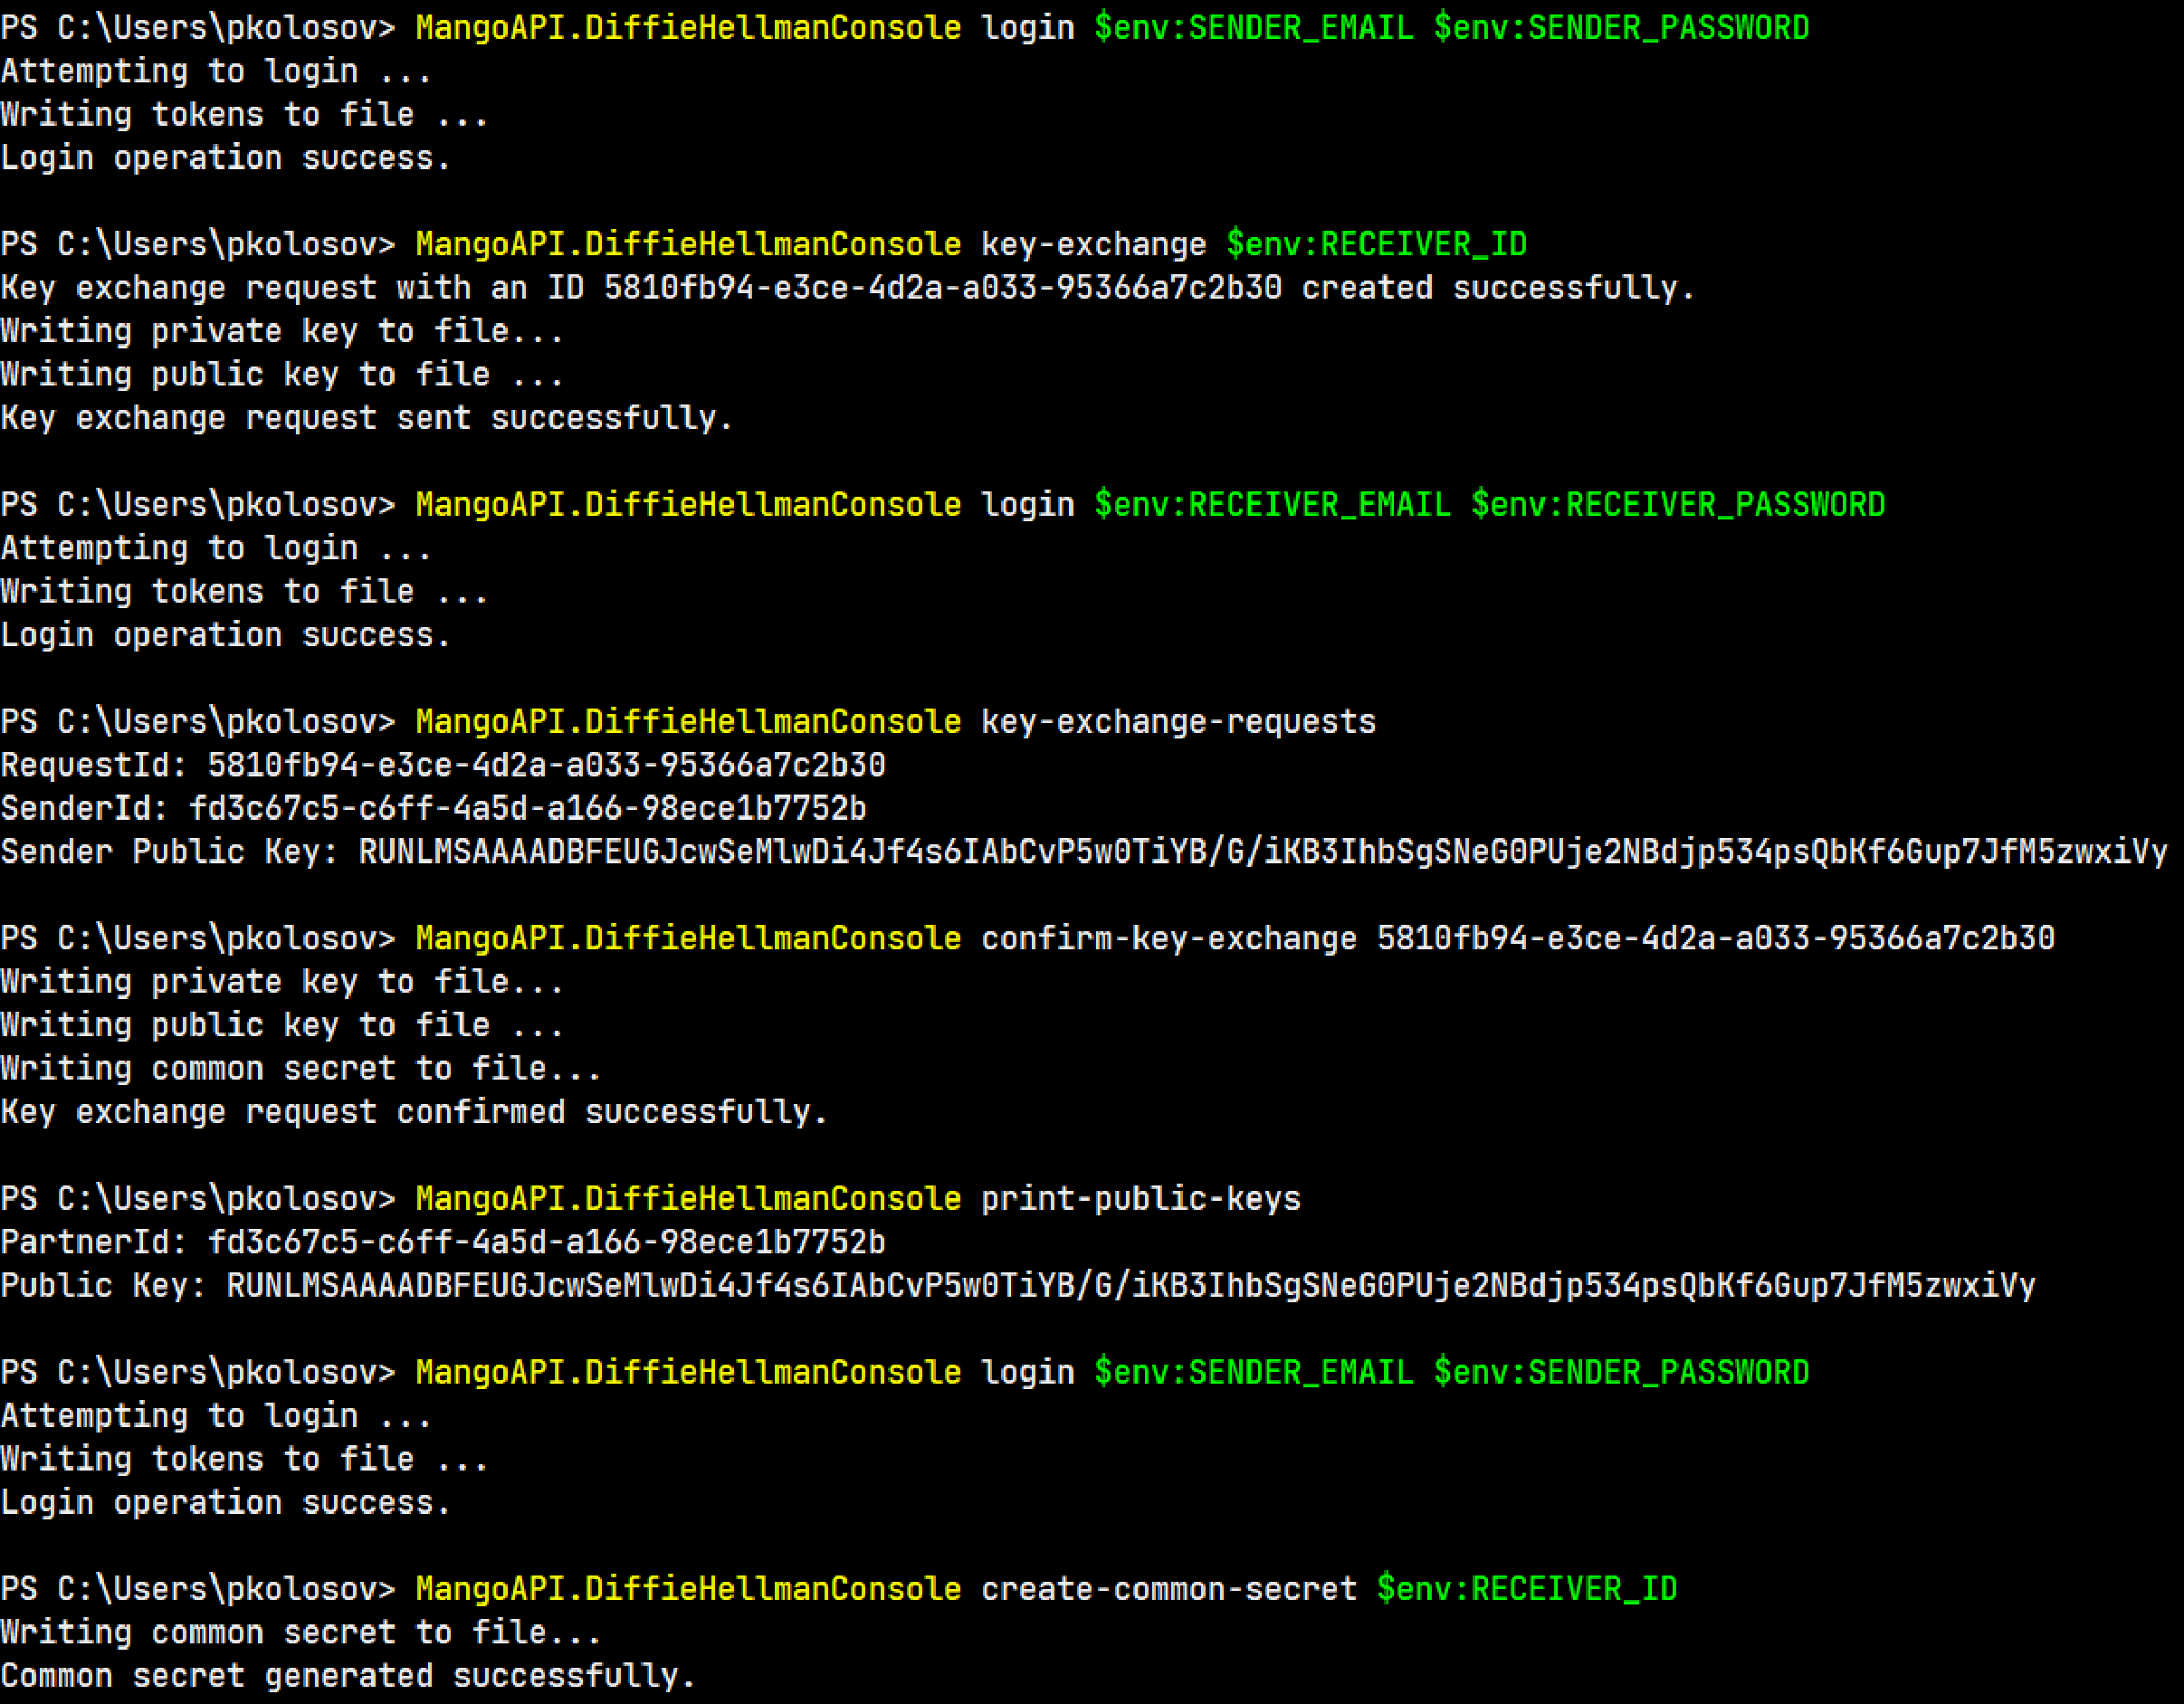
\includegraphics[width=1\textwidth]{Pictures/Diffie_Hellman_console_output}
        ~\caption{Diffie–-Hellman key exchange console output.}\label{fig:figure7}
    \end{figure}
    In order to repeat the outputs on the screenshot the user may reference to the resources
    \begin{itemize}
        \item API: \href{https://back.mangomessenger.company/swagger}{\texttt{https://back.mangomessenger.company/swagger}}
        \item Source: \href{https://github.com/MangoInstantMessenger/MangoMessengerAPI}{\texttt{https://github.com/MangoInstantMessenger/MangoMessengerAPI}}
    \end{itemize}
    Finally, both test accounts reached the same base 64 common secret.
    \begin{figure}[H]
        \centering
        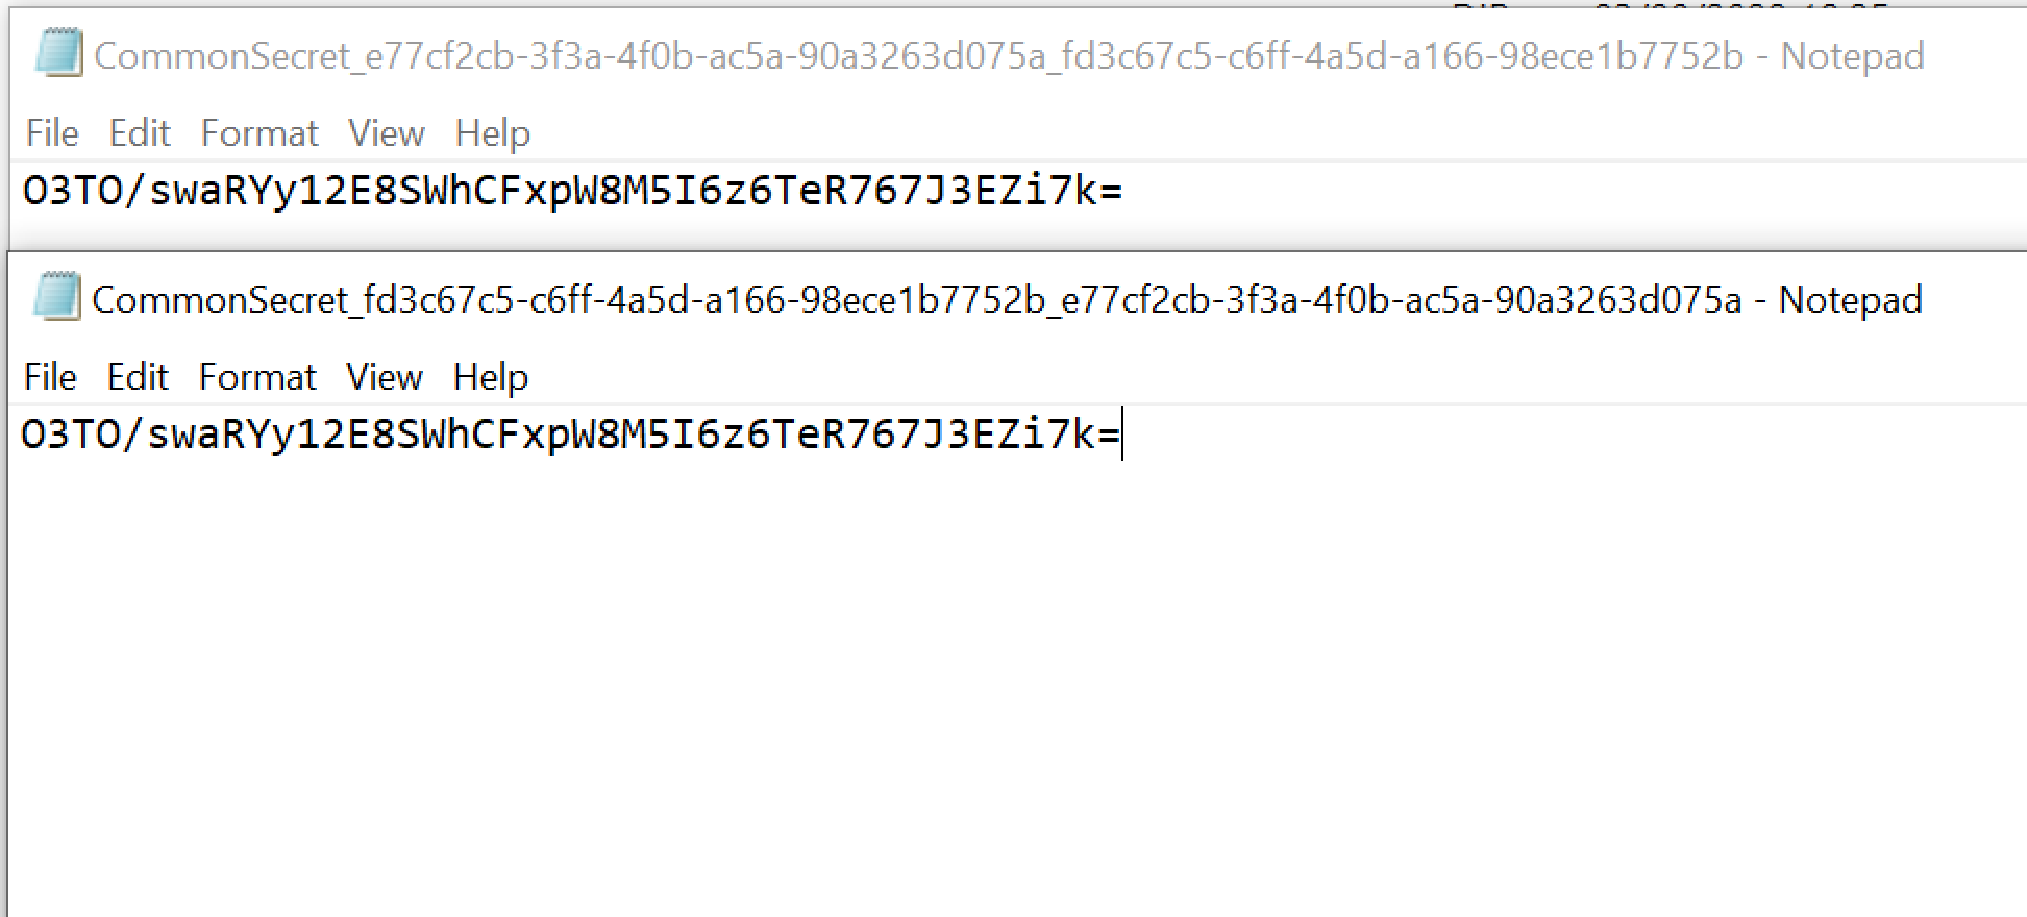
\includegraphics[width=1\textwidth]{Pictures/Same_common_secret}
        ~\caption{Common secrets.}\label{fig:figure2}
    \end{figure}

    \bibliographystyle{alpha}
    \bibliography{DiffieHellmanKeyExchangeReferences}

\end{document}
